\chapter{Laplacian Operator and Heat Kernel Formalism}

\section{Introduction to the Laplacian Formalism}
The formalism based on the Laplacian operator represents one of the most powerful and versatile mathematical representations for studying complex networks. This operator is not just an abstract matrix, but possesses a profound \textbf{physical meaning}: it represents the discrete generalization of the continuous Laplacian operator \( \Delta \) on a graph. It finds applications in describing spring systems, oscillatory dynamics, diffusion processes on graphs, and even Ricci flow on manifolds.

From a topological and structural perspective, the Laplacian matrix is fundamental because:
\begin{itemize}
    \item It allows for the identification of \textbf{disconnected components} in the network (the multiplicity of the zero eigenvalue corresponds to the number of connected components).
    \item It allows for the identification of network \textbf{communities}, typically by studying its eigenvalue spectrum (spectral clustering).
    \item It provides an optimal node coordinate set to \textbf{visualize a network} (graph and node embedding techniques, such as \textit{Laplacian eigenmaps}).
\end{itemize}

There are mainly two types of Laplacian operators associated with graphs: the \textit{oscillatory} and the \textit{diffusive} ones. In this section, we will focus on the former.

\subsection{From Continuous to Discrete: Notes on the Operator}
Before defining the Laplacian matrix, it is useful to draw a parallel with continuous analysis. A linear operator acting on a function (often calculated through an integral) can be discretized and represented as the product of a matrix and a vector.

In the continuous domain, the action of an integral operator on a function \( f(x) \) yields a new function \( g(y) \):
\[
    g(y) = \int L(x,y)f(x)dx
\]
In particular, for the Laplace operator \( \Delta \), the mapping is:
\[
    \Delta : f \rightarrow g = \Delta f
\]
Moving to the discrete case of a graph with \( N \) nodes, continuous functions become vectors \( \vec{x} \in \mathbb{R}^N \) (where each component \( x_i \) is the value of the function at node \( i \)). The continuous Laplacian operator \( \Delta \) is replaced by the Laplacian matrix \( L \), defining a linear mapping between discrete vector spaces (typically \( L: \mathbb{R}^N \rightarrow \mathbb{R}^N \)):
\[
    L : \vec{x} \rightarrow \vec{y} = L \cdot \vec{x}
\]

\subsection{Laplacian - Type 1 (Oscillatory)}
The type 1 Laplacian, called \textbf{oscillatory}, for a simple graph is defined as:
\[
    L = D - A
\]
where \( A \) is the adjacency matrix of the graph and \( D \) is the diagonal degree matrix, defined as:
\[
    D =
    \begin{pmatrix}
        k_1    & 0      & \dots  & 0      \\
        0      & k_2    & \dots  & 0      \\
        \vdots & \vdots & \ddots & \vdots \\
        0      & 0      & \dots  & k_N
    \end{pmatrix}
\]
with \( k_i \) representing the degree of node \( i \) (or, in the physical analogy, the local elastic constant).

A fundamental property of the Laplacian matrix \( L \) is evident from its \textbf{bilinear form}, which is proven to be positive semi-definite. For a generic vector \( \vec{x} \), we have:
\[
    \vec{x}^T L \vec{x} = \sum_{i \sim j} (x_i - x_j)^2 \geq 0 \quad \forall \vec{x}
\]
where the sum is over all edges of the graph (adjacent nodes \( i \sim j \)). Since this quadratic form is always non-negative, we can deduce that \textbf{all eigenvalues of \( \boldsymbol{L} \) are non-negative (\( \lambda_i \geq 0 \))}.

Furthermore, there is always at least one \textbf{zero eigenvalue} (\( \lambda_1 = 0 \)). For \( \vec{x}^T L \vec{x} = 0 \) to hold, all terms \( (x_i - x_j)^2 \) must be zero, which implies that \( x_i = x_j \) for every pair of connected nodes. Therefore, the eigenvector associated with the zero eigenvalue is the constant vector:
\[
    \vec{x}^T L \vec{x} = 0 \implies \vec{x} = \mathbf{1} = (1, 1, \dots, 1)^T
\]

In summary, the discrete Laplacian serves as an approximation of second derivatives. The operation \( \Delta f(x) \rightarrow L\vec{x} \) represents \textbf{second-order finite differences}. From a physical standpoint, if we imagine the nodes as unit masses and the edges as springs, the non-zero elements of the matrix, weighted by \( L_{ij} \), represent the \textbf{spring rigidity} and, consequently, the exchanged elastic forces.

\begin{example}[Springs on a 1D Lattice]
    To understand the origin of the term "oscillatory", let us consider a physical system of nodes connected by springs on a 1D lattice. Let \( x_i \) be the displacement of the \( i \)-th mass from its equilibrium position.

    According to Hooke's Law, the force exerted by the spring between node \( i \) and node \( i-1 \) is:
    \[
        F_{i} = -k(x_i - x_{i-1})
    \]
    assuming fixed boundary conditions (e.g., \( x_1 = x_N = 0 \)). The elastic potential energy associated with this single spring is:
    \[
        U_i = \frac{1}{2}k(x_i - x_{i-1})^2
    \]

    The total force \( F(x_i) \) acting on mass \( i \) is given by the sum of the forces exerted by the two adjacent springs:
    \[
        \begin{aligned}
            F(x_i) & = F_i - F_{i+1}                        \\
                   & = -k(x_i - x_{i-1}) + k(x_{i+1} - x_i) \\
                   & = -k(-x_{i-1} + 2x_i - x_{i+1})
        \end{aligned}
    \]
    Applying Newton's second law for a mass \( m \), we obtain the equation of motion:
    \[
        m\ddot{x}_i = F(x_i) \implies \ddot{x}_i = \frac{k}{m} \Delta x_i
    \]
    where the expression \( (-x_{i-1} + 2x_i - x_{i+1}) \) is exactly the one-dimensional discrete Laplacian operator \( \Delta x_i \).

    We can rewrite the entire system of differential equations in a compact matrix form:
    \[
        M \cdot \ddot{\vec{x}} = - L \cdot \vec{x}
    \]
    where \( M \) is a diagonal matrix of the "masses" (generally unit masses \( M = I \), but in more complex models they can represent specific parameters associated with each node). From here, isolating the acceleration, we obtain:
    \[
        \ddot{\vec{x}} = - M^{-1} \cdot L \cdot \vec{x} = - M^{-1} \cdot (I^T \cdot K \cdot I) \cdot \vec{x}
    \]
    \textit{Note on sign convention:} The formula can be reported omitting the minus sign (\( M \cdot \ddot{\vec{x}} = L \cdot \vec{x} \)). This happens because sometimes, depending on the reference text, the Laplacian is defined algebraically by absorbing the sign of the restoring force. The decomposition \( L = I^T \cdot K \cdot I \) (where \( I \) is the incidence matrix and \( K \) the diagonal stiffness matrix) clearly shows the positive semi-definite structure of the operator, confirming that it faithfully describes the oscillatory nature of the system.
\end{example}

\subsection{Physical Interpretation: Incidence Matrix, Gradient, and Divergence}
To deeply understand the physical meaning of the discrete Laplacian, we can express it through the \textbf{incidence matrix} \( I \). In a graph with \( N \) nodes and \( L \) links (edges), the incidence matrix \( I \) has dimensions \( L \times N \). It maps the \( N \)-dimensional node space to the \( L \)-dimensional link space.

In continuous real Euclidean space, the \textbf{gradient} operator \( \nabla \) maps a scalar function \( f \in \mathbb{R}^1 \) to a vector field in the variable domain \( \mathbb{R}^N \) (where \( N \) is the dimension of the space):
\[
    \nabla : f \rightarrow g = \nabla f = \left( \frac{\partial f}{\partial x}, \frac{\partial f}{\partial y}, \dots \right)
\]
In the discrete graph space, the incidence matrix \( I \) acts exactly as the discrete gradient. It maps a function defined on the nodes \( \vec{x} \in \mathbb{R}^N \) to a function defined on the edges \( \vec{y} \in \mathbb{R}^L \):
\[
    I : \mathbb{R}^N \rightarrow \mathbb{R}^L \implies \vec{y} = I \cdot \vec{x}
\]
Conversely, the transpose of the incidence matrix, \( I^T \) (dimensions \( N \times L \)), acts as the discrete \textbf{divergence}, mapping edge flows back to the nodes.

The standard unweighted Laplacian is therefore constructed as the product of the divergence and the gradient, which corresponds to the "square" of the incidence matrix:
\[
    L = I^T \cdot I
\]
Because it is constructed as \( I^T I \), the Laplacian is intrinsically a \textbf{positive semi-definite matrix}. Notably, the signs used inside \( I \) to define link orientations cancel out in \( L \); thus, the orientation of the links does not affect the final Laplacian matrix of an undirected graph.

For a weighted graph, we introduce a diagonal weight matrix \( G \). \textit{(Note: while the slides mention \( G \) as an \( N \times N \) matrix, mathematically, to satisfy the matrix multiplication \( I^T \cdot G \cdot I \), \( G \) must be an \( L \times L \) matrix representing the weights of the edges)}. The weighted Laplacian \( L_W \) is defined as:
\[
    L_W = I^T \cdot G \cdot I
\]
This perfectly mirrors the continuous definition of the Laplacian as the divergence of the gradient:
\[
    \nabla \cdot \nabla f = \Delta f = g = \sum_i \frac{\partial^2 f}{\partial x_i^2}
\]

\subsection{Bilinear Form as a Measure of Smoothness}
The bilinear form of the Laplacian evaluated for a generic vector \( \vec{x} \) (representing a signal or function on the nodes) maps \( \mathbb{R}^N \rightarrow \mathbb{R} \):
\[
    \vec{x}^T L \vec{x} = \sum_{i \sim j} (x_i - x_j)^2
\]
This discrete sum of squared differences is the exact equivalent of the \textbf{smoothness integral} (or Dirichlet energy) in the continuous domain. Using integration by parts, the continuous integral of a function multiplied by its Laplacian is:
\[
    \int f \cdot (\Delta f) dx = \left. f \cdot f' \right|_{\partial u} - \int \left( \frac{\partial f}{\partial x} \right)^2 dx
\]
Assuming the function \( f \) or its derivative \( f' \) vanishes at the boundary, the first term disappears. The integral of the squared gradient measures how much the function fluctuates.

In a more general manifold setting \( \mathcal{M} \), this smoothness measure \( \mathcal{S}(f) \) is defined as:
\[
    \mathcal{S}(f) \overset{\text{def}}{=} \int_{\mathcal{M}} |\nabla f|^2 d\mu = \int_{\mathcal{M}} f \Delta f d\mu = \langle \Delta f, f \rangle_{\mathcal{L}^2(\mathcal{M})}
\]
Therefore, the bilinear form in discrete graph space is a direct measure of function "smoothness". Given the spectral decomposition of \( L \), approximating a function using the first few eigenvectors (the \textbf{low-frequency modes}) guarantees maximal smoothness of the function over the graph. This principle is famously exploited in machine learning, such as in the Belkin-Niyogi semi-supervised learning framework (\textit{Laplacian Eigenmaps}).

\subsection{The Dirichlet Problem and Vibrating Membranes}
The eigenvalue problem of the Laplacian can be viewed as the discretized version of the \textbf{Dirichlet Problem}:
\[
    \Delta f = \lambda f
\]
where the function \( f \) is constrained to vanish at the edges of the region (boundary conditions).

A classic 2D physical example is a \textbf{vibrating membrane} (like a drumhead). In this context:
\begin{itemize}
    \item The \textbf{eigenvalues (\( \lambda \))} represent the \textbf{characteristic frequencies} of the membrane. Low values correspond to low frequencies (slow, smooth vibrations), and high values correspond to high frequencies (rapid, highly fluctuating vibrations).
    \item The \textbf{eigenvectors (\( f \))} represent the actual \textbf{vibrating modes} (the spatial shapes the membrane assumes while vibrating at those specific frequencies) on the "graph membrane".
\end{itemize}
It is important to note that a graph is a more general mathematical structure (a generalized manifold) and is not necessarily mappable into a simple 2D membrane.

\subsection{Isomorphism and Co-spectrality}
Solving the Dirichlet problem on a graph equates to finding the complete eigenvalue/eigenvector spectrum of its Laplacian. This leads to a fundamental question in spectral graph theory regarding \textbf{isomorphic} and \textbf{co-spectral} graphs.

Two graphs are \textit{co-spectral} if they share the exact same set of eigenvalues. A major question is whether:
\[
    \text{Co-spectral} \implies \text{Isomorphic?}
\]
In other words, given the spectrum of a network, can we univocally identify its specific topology?

This question was famously posed for the continuous case in 1966 by Mark Kac in the American Mathematical Monthly article: \textbf{"Can one hear the shape of a drum?"} (i.e., if you know all the resonant frequencies, do you know the drum's exact shape?).
\textit{(Note: The answer, both in the continuous case and for discrete graphs, was later proven to be "No" in general. There exist non-isomorphic graphs that share the same exact spectrum, meaning you cannot always perfectly reconstruct the network solely from its eigenvalues. However, the spectrum still provides massive amounts of structural information).}

\section{Spectral Properties of the Laplacian}

\subsection{The First Eigenvectors and Network Components}

The spectrum of the Laplacian matrix provides immediate and profound insights into the macroscopic structure of a network, starting with its smallest eigenvalues.

If a network consists of a \textbf{unique connected component}, there is exactly one zero eigenvalue (\( \lambda_1 = 0 \)). The corresponding eigenvector is the constant vector:
\[
    L \vec{x} = 0 \implies \vec{x} = (1, \dots, 1)^T
\]

If the network has \textbf{disconnected components} (often referred to as disjoint sub-networks or blocks), the multiplicity of the zero eigenvalue changes. Specifically, \textbf{there are as many null eigenvalues as there are disconnected components}.
Furthermore, the corresponding eigenvectors act as indicator vectors for these components: they have non-zero values strictly in correspondence to the nodes belonging to each specific component, and zeros elsewhere. For example, in a network with two disconnected blocks, the first two eigenvectors would look like:
\[
    \begin{aligned}
        \vec{x}_1 & = (1, \dots, 1, 0, \dots, 0, 0, \dots, 0)^T \\
        \vec{x}_N & = (0, \dots, 0, 0, \dots, 0, 1, \dots, 1)^T
    \end{aligned}
\]
By calculating the eigenvalues of the Laplacian, the number of null eigenvalues determines exactly how many disjoint subspaces exist. Subsequently, examining the non-null components of the corresponding relative eigenvectors allows us to define exactly which nodes belong to which disjoint subnetwork.

\textit{Note on Interpretation:} This clustering of nodes can also be interpreted through the lens of stochastic processes, specifically random walks on graphs, tying into the Perron-Frobenius theorem.

\begin{remark}[Computational Considerations]
    While this spectral approach yields exact results, it requires solving the full eigenvalue problem, which becomes computationally prohibitive for very large networks (e.g., \( 10^5 - 10^6 \) nodes).
    Alternatively, one can solve this recursively using the \textbf{Rayleigh functional minimization} to find eigenvalues up to \( \lambda > 0 \). However, one must be careful: since this is a numerical solution subject to floating-point approximations, one must define a threshold (how big must an eigenvalue be to be considered strictly \( > 0 \)?). In these cases, mathematical bounds on eigenvalues prove extremely useful.
    \textit{(Reference: Spectral Graph Theory, Fan Chung - available online).}
\end{remark}

\subsection{The Fiedler Number (\( \lambda_2 \)) and Algebraic Connectivity}

For a connected graph, the first eigenvalue is trivially zero. The \textbf{first non-zero eigenvalue} (typically denoted as \( \lambda_2 \), assuming eigenvalues are sorted in ascending order) is known as the \textbf{Fiedler number} (\( \lambda_2 > 0 \)). It is also widely referred to as the \textbf{algebraic connectivity} of the graph.

The Fiedler number has incredibly interesting properties related to:
\begin{itemize}
    \item Node clustering and community detection.
    \item Network display and optimal graph drawing.
    \item Various optimization problems.
    \item Synchronization dynamics and spreading processes on the network.
\end{itemize}
\textit{Example:} If we consider a network made of 2 full blocks (cliques) connected by a variable number of connecting links, the Fiedler number will grow as we add more links between the two blocks, reflecting a stronger overall connectivity.
\textit{(References: Spectral graph theory, Fan Chung CBMS 1997; Laplacian eigenvectors of graphs, Stadler Springer 2007).}

\subsection{Connectivity in Network Ensembles}

The specific value of the Fiedler number—especially when evaluated in relation to the maximum degree of the network and the total number of vertices \( n \)—gives global information on the overall robustness and connectivity of the network. As previously established, \( \lambda_2 = 0 \) if the network is disjoint.

For different families of standard graphs (network ensembles), the Fiedler value scales differently with the number of nodes \( n \):

\begin{table}[H]
    \centering
    \begin{tabular}{lc}
        \toprule
        \textbf{Graph Type} & \textbf{Fiedler Value (\( \lambda_2 \))} \\
        \midrule
        Path                & \( \Theta(1/n^2) \)                      \\
        Grid                & \( \Theta(1/n) \)                        \\
        3D Grid             & \( \Theta(n^{-2/3}) \)                   \\
        Expander            & \( \Theta(1) \)                          \\
        Binary Tree         & \( \Theta(1/n) \)                        \\
        Dumbbell            & \( \Theta(1/n) \)                        \\
        \bottomrule
    \end{tabular}
\end{table}

Notably, \textbf{Erdős–Rényi (E-R) random graphs} act as \textbf{expanders} (graphs that are sparse but highly connected) provided they have a sufficiently high link density.

\begin{figure}[H]
    \centering
    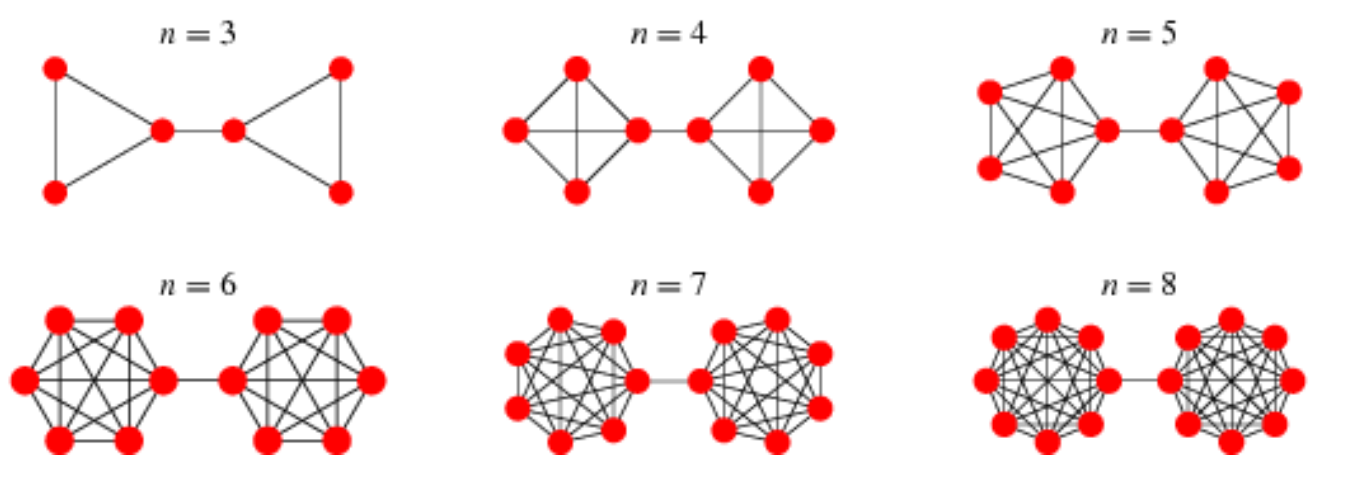
\includegraphics[width=0.8\textwidth]{img/dumbbell_evolution.png}
    \caption{Evolution of dumbbell graphs for a growing number of nodes \( n \) (from \( n=3 \) to \( n=8 \)). The Fiedler number decreases as the graph becomes more "bottlenecked" with a single link connecting two large cliques.}
\end{figure}

\begin{figure}[H]
    \begin{minipage}{0.5\textwidth}
        \centering
        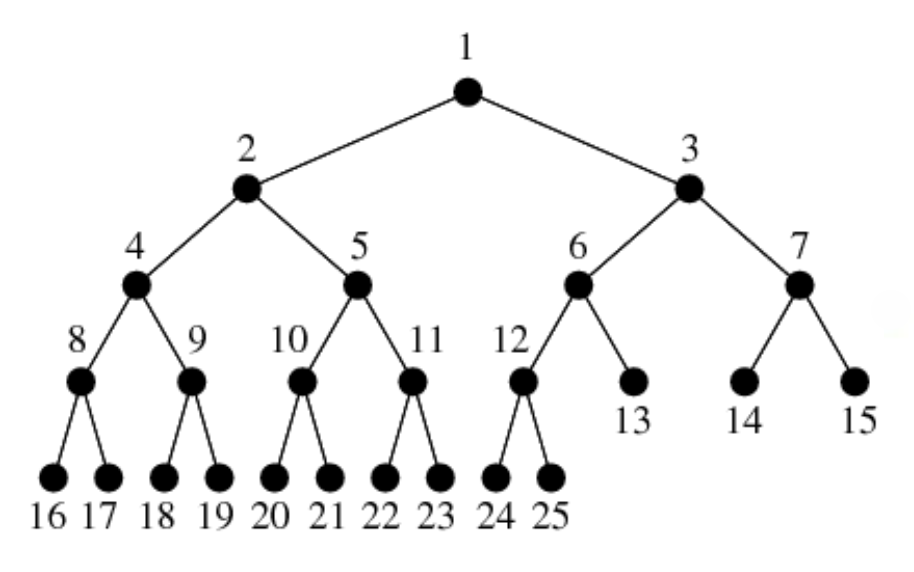
\includegraphics[width=0.8\textwidth]{img/binary_tree_graph.png}
    \end{minipage}\hfill
    \begin{minipage}{0.45\textwidth}
        \caption{A binary tree graph, which has a Fiedler number that scales as \( \Theta(1/n) \), reflecting its relatively poor connectivity compared to more densely connected graphs.}
    \end{minipage}
\end{figure}

\subsection{Graph Bipartitioning via the Fiedler Vector}

The Fiedler number provides a measure of connectivity: a "small" Fiedler eigenvalue indicates a poorly connected graph (e.g., a graph with a narrow bottleneck).

More importantly, the eigenvector associated with \( \lambda_2 \) — known as the \textbf{Fiedler vector} — gives us a powerful heuristic to divide the graph into \textbf{two parts} (bipartitioning). This is achieved simply by looking at the \textbf{sign} of its components.

Because Laplacian eigenvectors are orthogonal to each other, and the first eigenvector is the all-ones vector (all-positive), every subsequent eigenvector (including the Fiedler vector) \textbf{must have both positive and negative components} to satisfy orthogonality (\( \vec{x}_1 \cdot \vec{x}_2 = 0 \)).

By assigning nodes with a positive component in the Fiedler vector to one group, and nodes with a negative component to another, we effectively cut the graph along its weakest structural bottleneck.

For example, given a Fiedler vector:
\[
    \vec{x}_2 = (-0.3336, -0.3336, \dots, -0.2341, 0.2341, 0.3336, 0.3336, \dots)
\]
The nodes corresponding to negative values form one cluster, and those with positive values form the other.

\begin{figure}[H]
    \centering
    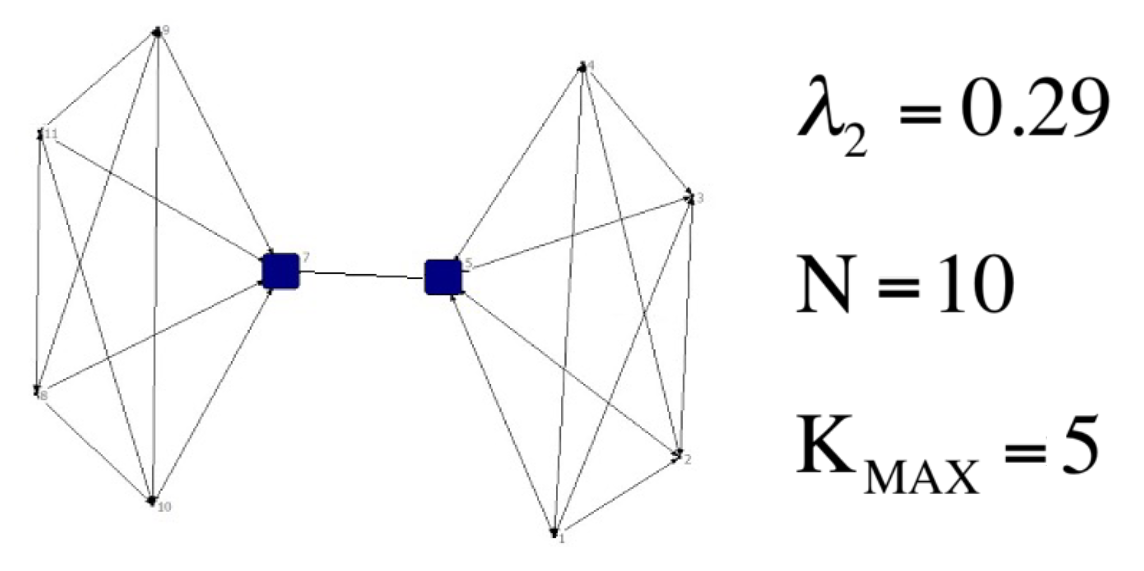
\includegraphics[width=0.8\textwidth]{img/bipartite_dumbbell.png}
    \caption{A bipartite dumbbell graph with \( N=10 \) nodes and a maximum degree \( K_{max}=5 \). The nodes are visually separated into two distinct clusters connected by a single central link, with a Fiedler number \( \lambda_2 = 0.29 \).}
\end{figure}

\subsection{Node Clustering: Two Main Strategies}

Following the concept of bipartitioning via the Fiedler vector, we can generalize the approach to divide the network into multiple communities. Historically and practically, there are two primary strategies for node clustering using the Laplacian spectrum:

\begin{enumerate}
    \item \textbf{Recursive Bi-partitioning:} This is the classical procedure (widely used since the 2000s). It consists of applying the Fiedler vector bipartitioning recursively. Once the network is divided into two subnetworks using \( \lambda_2 \), we compute the Laplacian for each new subnetwork and split them again using their respective Fiedler vectors, continuing until a desired number of clusters is reached or a stopping criterion is met.

    \item \textbf{Subspace Clustering (Spectral Embedding):} This is a more modern approach with many "variations on the theme". Instead of recursively cutting the graph, we select a \textbf{subspace of \( N \) eigenvectors} corresponding to the smallest non-zero eigenvalues. The components of these first \( N \) eigenvectors provide a new set of coordinates for each node, creating an \textbf{optimal \( N \)-dimensional embedding}. By mapping nodes into this smooth manifold space, we can then apply standard spatial clustering techniques (such as PCA, K-means, or hierarchical clustering) to group the nodes.
\end{enumerate}

\textit{Note on Embedding:} In the second strategy, taking the components of the first \( K \) eigenvectors of \( L \) effectively assigns a \( K \)-dimensional coordinate vector to each node. This is precisely what is meant by "graph embedding."

\begin{example}[Vibrational Analogy and Nodal Points]
    To better visualize how the signs of eigenvectors separate a network into clusters, we can return to a physical analogy: the vibrating rope (a 1D lattice of masses and springs).

    Imagine a rope fixed at both ends. The dynamics of this system map perfectly to the Laplacian formalism:
    \begin{itemize}
        \item \textbf{Eigenvalues} represent the resonant \textbf{frequencies} of the rope.
        \item \textbf{Eigenvectors} represent the \textbf{vibrational modes} (the standing wave patterns).
        \item \textbf{The sign of the eigenvector components} determines the position of the oscillation (whether a specific point on the rope is displaced "above" or "below" the resting axis).
    \end{itemize}

    The points where the eigenvector components cross zero are called \textbf{nodal points}. These nodal points physically separate different regions of the rope that are vibrating in synchrony (i.e., they have the same sign). In the context of a graph, these nodal points correspond to the "cut points" that separate clusters of nodes with positive and negative components in the Fiedler vector.

    \begin{figure}[H]
        \centering
        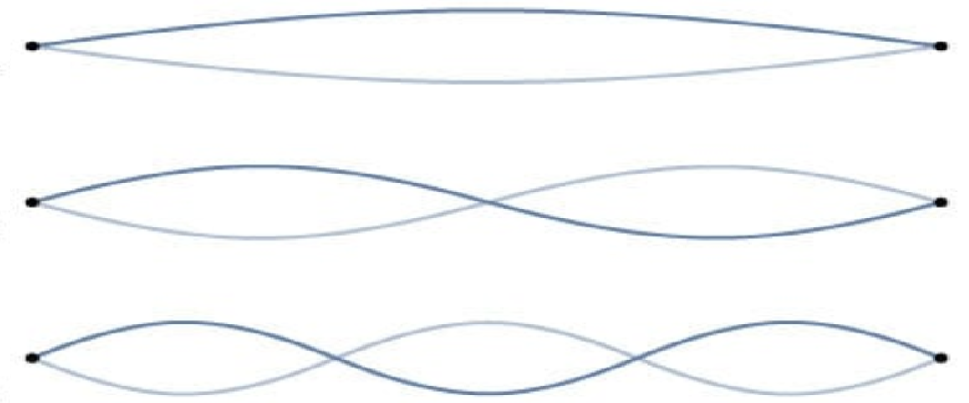
\includegraphics[width=0.8\textwidth]{img/stationary_waves.png}
        \caption{Visualization of standing waves on a vibrating rope. The nodal points (where the wave crosses the central axis) correspond to the sign changes in the eigenvector components, effectively separating different clusters of nodes in a graph.}
    \end{figure}
\end{example}

\subsection{Notes on Clustering, Manifolds, and Intrinsic Metrics}

In continuous real \( N \)-dimensional manifolds (like the rope or a metal plate), \textbf{nodal points} physically divide different regions of the manifold that are vibrating in synchrony (domains with the same sign).

However, if we are dealing with a pure \textbf{topological manifold} (a general complex network), we have a problem: we have no geometric idea of what a "region" is, because the graph lacks a spatial metric (distance between nodes is only topological, not physical).

We can resolve this if the network possesses an \textbf{intrinsic metric}. Good examples of this are found in computational biology, such as the contact map of a folded protein or DNA Hi-C data. In these cases, the nodes are sequentially ordered along a 1D chain (the amino acid sequence or the DNA strand). We can exploit this node ordering to index the graph and separate regions that share the same eigenvector sign in close proximity along the chain.
\textit{(Reference: Chen Bioinfo16, available in Virtuale).}

\subsection{The Second Eigenvector and Node Ordering}
Beyond clustering, the Fiedler vector (\( \vec{x}_2 \)) is extraordinarily useful for optimal \textbf{node ordering} and network visualization.

If we order the nodes of a network based on the sorted values of their components in the smallest non-zero eigenvector, we achieve a specific visual and structural optimization: we \textbf{reduce the length of the drawn links}.

Mathematically, the Laplacian bilinear form measures the sum of squared differences across connected nodes:
\[
    \vec{x}^T L \vec{x} = \sum_{i,j \text{ connected}} (x_i - x_j)^2
\]
Finding the eigenvectors of \( L \) is equivalent to finding the vectors \( \vec{x} \) that minimize the \textbf{Rayleigh quotient}:
\[
    \min \left( \frac{\vec{x}^T L \vec{x}}{||\vec{x}||^2} \right)
\]
\textit{(Note: On the original slide, the denominator is written as \( ||\vec{x} \cdot \vec{x}|| \), which conceptually represents the squared norm of the vector, typically denoted as \( ||\vec{x}||^2 \) or \( \vec{x}^T \vec{x} \)).}

This minimization process implicitly minimizes the \textbf{topological distances} between connected nodes.
The absolute minimum is achieved by the first eigenvector (\( \vec{x}_1 = \mathbf{1} \)), which yields \( \vec{x}^T L \vec{x} = 0 \). However, this is a \textit{trivial solution} because it places all nodes at the exact same coordinate (all-zero distances).

The second eigenvector (\( \vec{x}_2 \)) provides the first \textit{non-trivial} solution. By assigning these values to the nodes, connected nodes are pulled as close together as possible in a 1D space without collapsing into a single point.

\begin{example}
    Consider a simple linear graph of 5 nodes.
    The Fiedler vector for this specific topology assigns coordinates that space the nodes out symmetrically while keeping connected nodes adjacent:
    \[
        \vec{x}_2 = (-0.6015, \ -0.3717, \ 0.0000, \ 0.3717, \ 0.6015)^T
    \]
    By ordering the nodes according to these values, we naturally recover the optimal 1D layout of the chain.
    \begin{figure}[H]
        \centering
        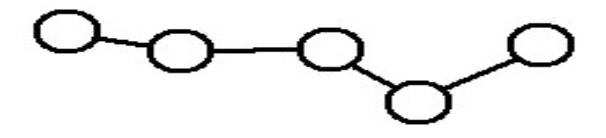
\includegraphics[width=0.8\textwidth]{img/chain_graph.png}
        \caption{A simple chain graph with 5 nodes. The Fiedler vector assigns coordinates that space the nodes symmetrically while keeping connected nodes adjacent.}
    \end{figure}
\end{example}

\subsection{Graph Visualization: The Center of Mass Approach}
A fundamental problem in graph visualization is determining optimal coordinates to draw the nodes so that the network structure is visually clear. A highly effective heuristic is to try to place each node as close as possible to the \textbf{center of mass} of its neighboring nodes.

Let \( x_i \) be the position of node \( i \). The center of mass of its neighbors, \( x_i^{CM} \), is computed by averaging their positions, weighted by the adjacency matrix \( A \):
\[
    x_i^{CM} = \frac{\sum_j A_{ij}x_j}{\sum_j A_{ij}}
\]
In matrix notation, recognizing that the denominator \( \sum_j A_{ij} \) is simply the degree of node \( i \) (which sits on the diagonal of the degree matrix \( D \)), we can write the vector of all center of masses as:
\[
    \vec{x}_{CM} = D^{-1} A \vec{x}
\]
Ideally, we want every node to sit exactly at the center of mass of its neighbors, meaning \( \vec{x} = \vec{x}_{CM} \). Setting this up yields:
\[
    \vec{x} = D^{-1} A \vec{x} \implies D\vec{x} = A\vec{x} \implies (D - A)\vec{x} = 0 \implies L\vec{x} = 0
\]
This shows that finding these exact coordinates is equivalent to finding the null space of the Laplacian. As we know, the exact solution to \( L\vec{x} = 0 \) is the first eigenvector (\( \lambda = 0 \)), which is the constant vector \( \vec{x} = \mathbf{1} \). However, this is a \textbf{trivial solution}: it places all nodes at the exact same geometric point, which is useless for visualization.

Since we cannot use the exact solution, we reframe the problem as an extremal problem: we want to minimize the deviation from this ideal state. This leads us back to the \textbf{minimization of the Rayleigh functional}:
\[
    \min \left( \frac{\vec{x}^T L \vec{x}}{||\vec{x}||^2} \right)
\]
\textit{(Note: As in previous slides, the denominator represents the squared norm of the vector, denoted in the slide as \( \vec{x} \cdot \vec{x} \)).}

Because the first eigenvector (\( \lambda_1 = 0 \)) gives the trivial overlapping solution, we look at the \textbf{second eigenvector} (\( \lambda_2 \), the Fiedler vector), which provides the \textbf{next position of minimum}. It gives us the optimal non-trivial 1D coordinates to separate the nodes while keeping connected neighbors as close together as possible.

\subsection{Graph Visualization: Spring-Force Layout}
Another highly intuitive and widely used method for graph drawing expands directly upon the vibrational analogy: the \textbf{spring-force layout} (or force-directed graph drawing).

In this paradigm, the Laplacian graph is explicitly interpreted as a dynamic physical system:
\begin{itemize}
    \item \textbf{Links} act as \textbf{springs} pulling connected nodes together.
    \item \textbf{Edge Weights} represent the \textbf{spring stiffness} (stronger weights = stronger pull).
    \item \textbf{Node Mass} can be assigned based on node features, providing \textbf{"inertia"} that dictates how quickly a node moves through the simulation space.
\end{itemize}

If we only used springs, the entire graph would collapse into a single point (the trivial solution again). To stabilize the simulation and create an aesthetically pleasing visualization, \textbf{Coulombian repulsive forces} are usually added between \textit{all} pairs of nodes (treating nodes like equally charged particles).
The simulation runs until the system reaches mechanical equilibrium—where the attractive spring forces of the links balance the global repulsive forces.

\textit{Example:} This method is excellent for untangling complex structures and works perfectly to reveal the underlying geometry of 2D or 3D lattices, or distinct clusters in a 2-block graph.

\subsubsection{Summary: Applications of the Graph Laplacian}
To conclude this chapter, the Laplacian operator is a cornerstone of complex network analysis due to its deep connection to the structural topology. Its primary applications include:
\begin{itemize}
    \item \textbf{Identifying disconnected components} of a graph (counting the number of zero eigenvalues).
    \item \textbf{Node sorting and ordering} (revealing underlying intrinsic metrics and minimizing topological distances).
    \item \textbf{Clustering and Bipartitioning/Multi-partitioning} by utilizing the "main modes" of the Laplacian (the first few non-trivial eigenvectors, especially the Fiedler vector).
    \item \textbf{Network visualization} (using spectral embeddings or driving spring-force layouts).
    \item \textbf{Node and link centrality} (using spectral properties to measure the relative importance or bottleneck nature of specific network elements).
\end{itemize}

\section{Spectral Centrality (SC)}

\subsection{Network Deformation and Spectral Perturbation}
A powerful application of the Laplacian framework is the evaluation of node and edge importance through \textbf{Spectral Centrality (SC)}. We consider the Laplacian matrix \( L \) of a symmetrical (undirected) network.

The core idea is to apply a \textbf{deformation} to the network. A deformation consists of making the weight of a specific link, or all the links connected to a specific node or subgraph, go to zero (effectively weakening or removing them).

This structural deformation naturally induces a \textbf{perturbation} on the spectrum of the Laplacian (its eigenvalues and eigenvectors). The fundamental principle of Spectral Centrality is: \textbf{the more important the link, node, or subgraph is to the overall network structure, the greater the resulting perturbation on the spectrum}.

\textit{Example:} If we remove a cutpoint (a node whose removal disconnects the graph) or a bridge (a critical connecting link), the network breaks into multiple components. Mathematically, this immediately zeroes out the Fiedler number (\( \lambda_2 \rightarrow 0 \)), representing a massive spectral perturbation.

\subsection{K-Spectral Centrality: Continuous Approach}
We can formalize a family of centralities by looking at the continuous derivative of the \( k \)-th Laplacian eigenvalue with respect to a deformation induced by a subset \( B \) (where \( B \) can be a link, a node, or an entire subgraph).

The continuous \( k \)-spectral centrality of subset \( B \) is defined as the absolute rate of change of the eigenvalue:
\[
    S^k_B = |\lambda'_k(0)|
\]
where \( \vec{v}^k \) is the \( k \)-th eigenvector, and the derivative of the eigenvalue evaluated at the unperturbed state (0) is:
\[
    \lambda'_k(0) = \sum_{ij} C_{ij}
\]
Here, the matrix \( C \) is defined as \( C = FL'(0)F \), and \( F \) is a diagonal matrix whose entries are given by the components of the unperturbed eigenvector, \( v_k(0) \).

From this continuous framework, we can derive specific, easy-to-compute centrality formulas for individual network elements:
\begin{itemize}
    \item \textbf{Edge Centrality} (for the link between nodes \( i \) and \( j \)):
          \[
              s^k_{ij} = \left| v^k_i(0) - v^k_j(0) \right|
          \]
    \item \textbf{Node Centrality} (for node \( i \), aggregating the impact on all its connections weighted by the adjacency matrix \( A \)):
          \[
              s^k_i = \sum_j A_{ij} \left[ v^k_i(0) - v^k_j(0) \right]^2
          \]
\end{itemize}

\subsection{K-Spectral Centrality: Discrete Approach}
Alternatively, we can measure spectral centrality using a discrete approach. Instead of calculating continuous derivatives, we physically perturb the network by explicitly \textbf{removing} network elements (a link, a node, or a subnetwork). This conceptual approach is similar to how we calculate the drop in Network Efficiency to find Betweenness Centrality (BC).

After removing the element, we calculate the discrete variation of the Fiedler value (or any \( k \)-th eigenvalue):
\[
    \Delta F = F - F'
\]
\[
    \Delta\lambda^{(k)} = \lambda^{(k)} - \lambda^{(k)'}
\]
where the prime denotes the value in the perturbed network.

\textbf{The physical meaning of \( k \):} The choice of the specific eigenvalue sets the system \textbf{scale} (i.e., the "frequency") at which we want to measure the perturbation. Lower eigenvalues (\( k=2, 3 \)) measure the impact on global macroscopic structures, while higher eigenvalues measure the impact on local, highly fluctuating topological features.

\subsection{Applications: Time Series and Biological Networks}
Spectral Centrality proves extremely useful in real-world, data-driven networks.

\textbf{Networks from Time Series:}
Consider a network generated from the S\&P 500 financial time series at a daily scale. We start with the time correlation matrix \( C_{ij} \) between assets. We can map this to a distance metric:
\[
    s_{ij} = \sin(\arccos(C_{ij})/2),
\]
then convert it into an adjacency matrix using a Gaussian kernel:
\[
    A_{ij} = e^{- \frac{s_{ij}^2}{\sigma^2}}.
\]
\begin{figure}[H]
    \centering
    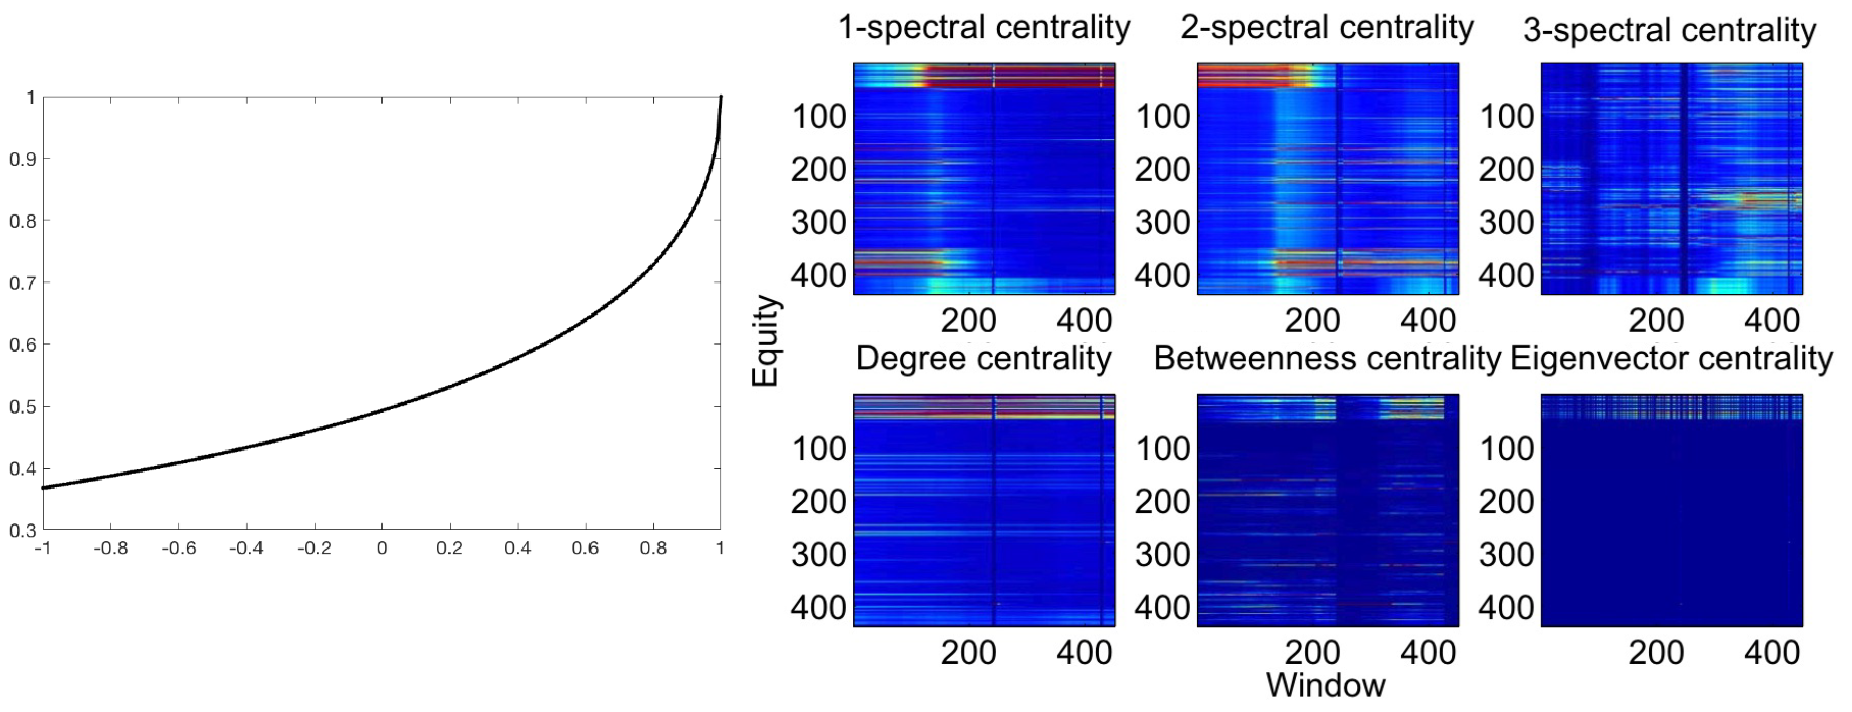
\includegraphics[width=0.8\textwidth]{img/sp500_correlation.png}
    \caption{Plot of correlation for the S\&P 500 assets on a daily scale (left), and the resulting heatmaps comparing 1-spectral, 2-spectral, and 3-spectral centralities against Degree, Betweenness, and Eigenvector centralities across different equity windows (dx).}
\end{figure}

\begin{example}[Spectral Centrality vs. Efficiency (Biological Example)]
    When studying complex biological networks, different metrics capture different systemic properties.

    In the context of the immune system:
    \begin{itemize}
        \item \textbf{Efficiency \( E \)} provides an \textbf{evolutionary} ranking (identifying nodes critical to the innate, baseline structural immune system).
        \item \textbf{Spectral Centrality \( SC \)} provides a \textbf{functional} ranking (identifying nodes that dynamically drive specific processes, like hematopoiesis).
    \end{itemize}
    \begin{figure}[H]
        \centering
        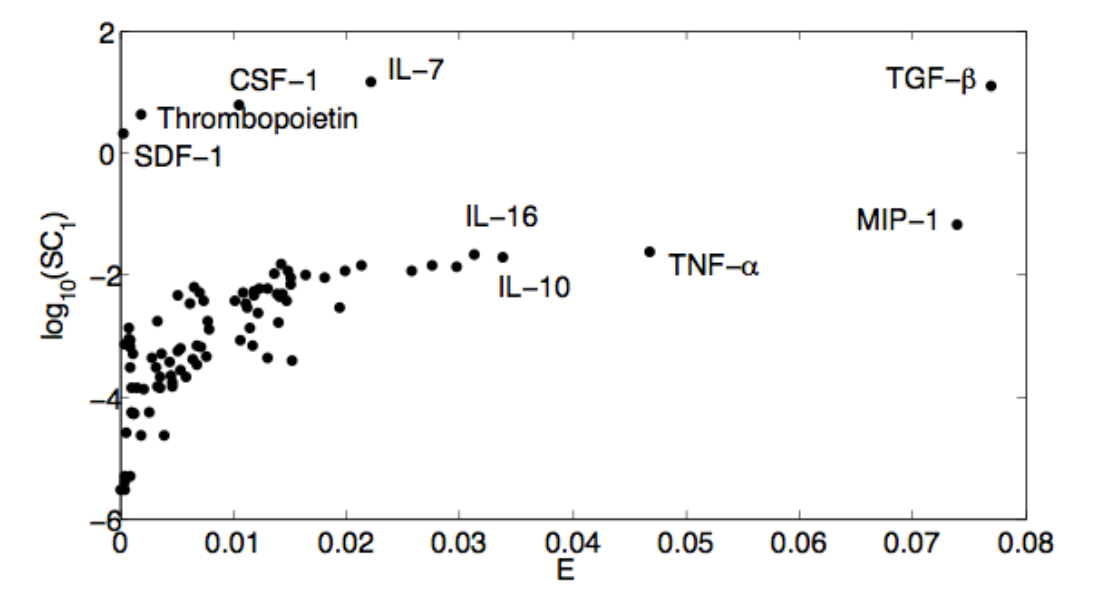
\includegraphics[width=0.8\textwidth]{img/biological_SC_E.png}
        \caption{Scatter plot comparing Spectral Centrality SC1 (log scale) vs. Efficiency E for biological immune system markers.}
    \end{figure}
\end{example}

\subsubsection{Important Notes on Spectral Centrality}
To correctly apply and interpret Spectral Centrality, a few key properties must be kept in mind:
\begin{itemize}
    \item \textbf{Correlation with other metrics:} For \textbf{sparse networks}, SC strongly correlates with standard centrality measures (like Degree or Betweenness).
    \item \textbf{Unique value in dense networks:} SC shines and diverges from standard measures when applied to \textbf{dense and weighted} networks, providing unique insights that simple path-based metrics miss.
    \item \textbf{Mathematical constraints:} The SC formalism strictly applies to \textbf{symmetrical} (undirected) networks. This is a mathematical requirement necessary to guarantee that the Laplacian matrix has real eigenvalues and a complete basis of real eigenvectors.
\end{itemize}

\section{Diffusive and Normalized Laplacians}

While the standard oscillatory Laplacian (\( L = D - A \)) is foundational, the influence of highly connected nodes (hubs) can sometimes dominate its spectrum. To address this and to model different physical phenomena, we introduce two alternative formulations: the diffusive and the normalized Laplacians.

\subsection{Laplacian Type 2: The "Diffusive" Laplacian}
If we take the standard Laplacian \( L \) and divide each of its columns by the degree of the respective node, we obtain a new matrix. This operation is equivalent to post-multiplying \( L \) by the inverse of the degree matrix, \( D^{-1} \).

The inverse degree matrix is a diagonal matrix defined as:
\[
    D^{-1} =
    \begin{pmatrix}
        1/k_1  & 0      & \dots  & 0      \\
        0      & 1/k_2  & \dots  & 0      \\
        \vdots & \vdots & \ddots & \vdots \\
        0      & 0      & \dots  & 1/k_N
    \end{pmatrix}
\]

We define the Type 2 Laplacian (often denoted as \( L' \) or \( L^{(2)} \)) as:
\[
    L^{(2)} = (D - A) \cdot D^{-1} = I - A \cdot D^{-1} = -T
\]
By performing this division, we effectively convert the adjacency information into a \textbf{stochastic transition matrix} \( T \) (also known as a random walk matrix). In this formulation:
\begin{itemize}
    \item The transition probability between states is always \( \geq 0 \).
    \item The total probability of transition from each state sums exactly to \( 1 \) (conservation of probability).
\end{itemize}

This matrix governs the dynamics of diffusion or random walks on the network. The evolution of a probability distribution \( p(t) \) over the nodes can be written as a finite difference equation:
\[
    \frac{p(t + \Delta t) - p(t)}{\Delta t} = T \cdot p(t)
\]

\textit{Crucial Note:} The elastic (oscillatory) and diffusive Laplacian operators are fundamentally different matrices. Most notably, because \( L^{(2)} \) is generally asymmetric, \textbf{they do not have the same eigen spectrum}.

\subsection{Laplacian Type 3: The "Normalized" Laplacian}
To retain the mathematical benefits of a symmetric matrix while still mitigating the overwhelming "weight" of high-degree nodes on the diagonal, we use the \textbf{Normalized Laplacian} (\( L^{(3)} \)).

Instead of dividing only the columns, we rescale the matrix symmetrically by pre- and post-multiplying by \( D^{-1/2} \) (where \( D^{-1/2} \) is the diagonal matrix with entries \( 1/\sqrt{k_i} \)):
\[
    L^{(3)} = D^{-\frac{1}{2}} L D^{-\frac{1}{2}} = I - D^{-\frac{1}{2}} A D^{-\frac{1}{2}}
\]

Because of this symmetric rescaling, \( L^{(3)} \) admits solutions that are explicit functions of the node degrees. If we look at the bilinear form:
\[
    \vec{x}^T L \vec{x} = \vec{x}^T D^{\frac{1}{2}} D^{-\frac{1}{2}} L D^{-\frac{1}{2}} D^{\frac{1}{2}} \vec{x} = (\vec{x}')^T L^{(3)} \vec{x}'
\]
where we define a transformed state vector \( \vec{x}' = D^{1/2} \vec{x} \).

Recall that for the standard Laplacian, the stationary state (trivial eigenvector for \( \lambda = 0 \)) is the constant vector \( \vec{1} \). For the normalized Laplacian, this stationary eigenvector transforms into a function of the square root of the node degrees:
\[
    \vec{x}'_{ST} = D^{\frac{1}{2}} \vec{1} = \left( \sqrt{k_1}, \sqrt{k_2}, \dots, \sqrt{k_N} \right)^T
\]

\subsection{Similarity Between Laplacian 2 and 3}
Although \( L^{(2)} \) is asymmetric and \( L^{(3)} \) is symmetric, they are deeply mathematically connected. The normalized Laplacian 3 is \textbf{similar} (in terms of matrix algebra) to the diffusive Laplacian 2.

We can prove this by rearranging the terms of \( L^{(3)} \):
\[
    \begin{aligned}
        L^{(3)} & = D^{-\frac{1}{2}} \cdot L \cdot D^{-\frac{1}{2}}                        \\
                & = D^{-\frac{1}{2}} \cdot (L \cdot D^{-1} \cdot D) \cdot D^{-\frac{1}{2}} \\
                & = D^{-\frac{1}{2}} \cdot (L \cdot D^{-1}) \cdot D^{\frac{1}{2}}          \\
                & = D^{-\frac{1}{2}} \cdot \left( L^{(2)} \right) \cdot D^{\frac{1}{2}}
    \end{aligned}
\]
Because \( L^{(3)} \) can be written as \( P^{-1} L^{(2)} P \) (where \( P = D^{1/2} \)), this constitutes a \textbf{similarity transform}.

The physical and structural consequence of this similarity is profound: \textbf{Laplacian 2 and Laplacian 3 possess the exact same spectrum of eigenvalues}. Their eigenvectors are also directly related, differing only by a \textbf{linear rescaling} (multiplication by the diagonal square root of the degree sequence, \( D^{1/2} \)).

\subsection{Summary Comparison: The Three Laplacians}
To synthesize the different formulations presented in this chapter:

\begin{enumerate}
    \item \textbf{Type 1 - Oscillatory (\( L = D - A \)):}
          \begin{itemize}
              \item \textbf{Properties:} Symmetric, positive semi-definite.
              \item \textbf{Physical Analogy:} Systems of springs, elastic forces, vibrating membranes. It models the minimization of energy and topological distances.
              \item \textbf{Quirk:} The spectrum is heavily bounded and influenced by the maximum degree (\( k_{\text{max}} \)) of the network. Large hubs dominate the eigenvalues.
          \end{itemize}

    \item \textbf{Type 2 - Diffusive/Random Walk (\( L^{(2)} = L D^{-1} \)):}
          \begin{itemize}
              \item \textbf{Properties:} Generally \textbf{asymmetric}.
              \item \textbf{Physical Analogy:} Stochastic processes, Markov chains, random walks, and heat/fluid diffusion. It models the flow of probability from one node to its neighbors.
              \item \textbf{Quirk:} Because it is asymmetric, its eigenvectors are not naturally orthogonal, making some spectral clustering algorithms harder to apply directly, though it perfectly describes transition rates.
          \end{itemize}

    \item \textbf{Type 3 - Normalized (\( L^{(3)} = D^{-1/2} L D^{-1/2} \)):}
          \begin{itemize}
              \item \textbf{Properties:} Symmetric, positive semi-definite.
              \item \textbf{Physical Analogy:} A mathematical "best of both worlds." It normalizes the topological space, treating nodes more equally regardless of their degree.
              \item \textbf{Quirk:} Its eigenvalues are strictly bounded between \( 0 \) and \( 2 \). It shares the identical spectrum of the diffusive Laplacian (capturing the same diffusion dynamics) but remains symmetric, making it the preferred matrix for modern spectral clustering and graph neural networks.
          \end{itemize}
\end{enumerate}
